\documentclass[12pt]{article}
\usepackage{graphicx} % Required for inserting images
% \usepackage{adjustbox}
\usepackage[margin=1in]{geometry}
\usepackage{graphicx}
\usepackage{amsmath}
\usepackage{mathtools}
\usepackage[version=4]{mhchem}
\usepackage{siunitx}
\usepackage{longtable,tabularx}
\setlength\LTleft{0pt} 
\newcommand{\HRule}{\rule{\linewidth}{0.5mm}}
\usepackage{longtable,tabularx}
\usepackage{multirow}
\usepackage{hyperref}
\usepackage[capitalise]{cleveref}
\usepackage{nomencl}
\usepackage{longtable}
\usepackage{textcomp}
\usepackage{listings}
\usepackage{matlab-prettifier}
\usepackage{float}
\usepackage{pdfpages}
\usepackage{booktabs}
\usepackage{adjustbox}
\usepackage[framed,numbered,autolinebreaks]{mcode}
\usepackage{framed}
\usepackage{multicol}
\usepackage{hyperref}
\hypersetup{
    colorlinks=true,
    linkcolor=black,
    filecolor=magenta,      
    urlcolor=cyan,
    citecolor=black,
    pdftitle={Overleaf Example},
    pdfpagemode=FullScreen,
    }

\usepackage{stackengine}
\newcommand\barbelow[1]{\stackunder[1.2pt]{$#1$}{\rule{.8ex}{.075ex}}}


\usepackage[makeroom]{cancel}

% \documentclass[border=3pt,tikz]{standalone}
% \usepackage{physics}
\usepackage{tikz}
\usepackage{tikz-3dplot}
\usepackage[outline]{contour} % glow around text
\usepackage{xcolor}
\usepackage{pgffor}

\colorlet{veccol}{green!50!black}
\colorlet{projcol}{blue!70!black}
\colorlet{myblue}{blue!80!black}
\colorlet{myred}{red!90!black}
\colorlet{mydarkblue}{blue!50!black}
\tikzset{>=latex} % for LaTeX arrow head
\tikzstyle{proj}=[projcol!80,line width=0.08] %very thin
\tikzstyle{area}=[draw=veccol,fill=veccol!80,fill opacity=0.6]
\tikzstyle{vector}=[-stealth,myblue,thick,line cap=round]
\tikzstyle{unit vector}=[->,veccol,thick,line cap=round]
\tikzstyle{dark unit vector}=[unit vector,veccol!70!black]
\usetikzlibrary{angles,quotes} % for pic (angle labels)
\contourlength{1.3pt}

\renewcommand{\thesection}{\Roman{section}} 
\renewcommand{\thesubsection}{\thesection.\alph{subsection}}

\title{ASEN 5212 Composites Final Project}
\author{Bryce Pfuetze}
\date{May 2025}

\begin{document}

\begin{titlepage}

\center
 
\textsc{\Large University of Colorado - Boulder}\\[.75cm] 
\vspace{-1em}
\textsc{\large ASEN 5212\\Composite Structures and Materials}\\[0.25cm]
% \vspace{-.1em}
% \textsc{\large Matrix Methods}\\[0.25cm]

\HRule \\[0.2cm]
{ \huge \bfseries Light in-Organic Laminates (LOL)  \\[0.25cm]}
\HRule \\[.5cm]

\begin{minipage}{0.70\textwidth}
\begin{flushleft} \large
\renewcommand{\thempfootnote}{\fnsymbol{mpfootnote}}
\emph{Authors:}\\  Claire Kent \\ Bryce Pfuetze \\ Samuel Hatton
 % Bryce \textsc{Pfuetze} \\
 % Samuel \textsc{Hatton} \\
 % Bryce Pfuetze \\
 % Samuel Hatton \\
\end{flushleft}
\end{minipage}
~
\begin{minipage}{0.25\textwidth}
\begin{flushright} \large
% \emph{Lab Instructors:} \\ 
% first \textsc{last} \\
{\large 10 May 2025}\\[1.5em]
\end{flushright}
\end{minipage}\\[1em]

% \large \textit{Lab}: Section 000\\[1em]

% {\large 6 December 2022}\\[.75em] 

\HRule \\[4em]

\begin{abstract}
This report explores the process of designing lightweight laminate composites for target stiffness and strength criteria. Within the design space, we are able to vary the number of unidirectional laminas $n$, the orientation of each lamina $\theta$, and fiber volume fraction within the range $0.4\leq V_f\leq0.65$. This analysis explores three cases: designing for stiffness, designing for strength, and designing for both stiffness and strength. In each case, the objective is to meet or exceed the prescribed performance requirements while minimizing the mass per unit area. Our approach is to first vary $n$ and $\theta$ to determine a set of candidate laminates. With the candidates in hand, we can then vary $V_f$ to determine the lightest laminate within our selection that successfully achieves the performance requirements. 
\end{abstract}



\vfill


\includegraphics[width=0.65\textwidth]{CU_Engineering (1).jpg}
%\newpage
%\pagenumbering{gobble}  
%\tableofcontents
\end{titlepage}

\section{Introduction}
For this project, our objective was to design a laminate that satisfied a given set of stiffness and/or strength criteria while also remaining as light as possible. The necessary material properties and failure properties of the carbon fibers and the epoxy matrix were given (Table \ref{tab:matprop}). Additional constraints included a fixed fiber volume fraction range of $0.4\leq V_f\leq0.65$, uniform volume fraction across each lamina, and a defined relationship between lamina thickness $t$ and $V_f$. Our unconstrained design variables were the number of laminas $n$ and fiber orientation $\theta$. 

\begin{table}[H]
    \centering
    \begin{tabular}{|c|c|c|}
        \hline
         & Fibers & Matrix\\
         \hline
         & $E_{1f}=270GPa$ & $E_m=3.5 GPa$\\
         & $E_{2f}=14 GPa$ & $-$\\
        Material Properties & $G_{12f}=10 GPa$ & $-$\\
         & $\nu_{12f}=0.22$ & $\nu_m=0.37$\\
         &  $\rho_f=1750\frac{kg}{m^3}$& $\rho_m=1200\frac{kg}{m^3}$\\
         \hline
         & & $F_{mt}=120 MPa$\\
        Failure Properties & $\varepsilon_f^u=0.01$ & $F_{mc}=150 MPa$\\
         & & $F_{ms}=80 MPa$\\
         \hline 
    \end{tabular}
    \caption{Material and failure properties of fibers and matrix}
    \label{tab:matprop}
\end{table}

When considering the mass of the laminate, $n$ and $V_f$ have the most direct effect. Increasing $n$ simply means adding more plies and therefore more material. The relationship between $t$ and $V_f$ is defined in Equation \ref{eq:tv}: the amount of fiber per lamina is held constant, and so lamina thickness varies proportionally with volume fraction. As such, an increase in $V_f$ means a decrease in matrix material but no change in fiber material, so higher volume fraction lamina have less mass. As seen in Figure \ref{fig:massChange}, $n$ has a much greater effect than $V_f$ on areal mass. Because of this, we primarily optimized primarily for a low $n$, focusing on increasing $V_f$ once a satisfactory laminate was found. This strategy does result in viable composite designs, but it is likely not sufficient to produce the lightest designs. It is likely that there exist lamina with more, lighter layers than our chosen solutions that also satisfy the design criteria.

Considering the physical properties of the laminate is a more complex process. Stiffness and strength properties depend heavily on $\theta$ values for each lamina and how they are combined. For axial stiffness $A_{xx}$, the primary considerations are the values of $\theta$ and how many plies of each angle are present. Position within the laminate has no effect. The same cannot be said for bending stiffnesses $D_{xx}$ and $D_{yy}$. Plies close to the neutral axis contribute less to bending stiffness, so position within the laminate matters. This is made clear when evaluating the expressions that define axial and bending properties in the ABD matrix. 

% \begin{multicols}{2}
%     \begin{equation}
%         A_{ij}=\sum^n_{k=1}Q^k_{ij}(z_k-z_{k-1})
%     \end{equation}
%     \begin{equation}
%         D_{ij}=\frac{1}{3}\sum^n_{k=1}Q^k_{ij}(z_k^3-z_{k-1}^3)
%     \end{equation}
% \end{multicols}

\begin{align}
    A_{ij}=\sum^n_{k=1}Q^k_{ij}(z_k-z_{k-1}) \\
    D_{ij}=\frac{1}{3}\sum^n_{k=1}Q^k_{ij}(z_k^3-z_{k-1}^3)
\end{align}

In the definition of $A_{ij}$, $z_k-z_{k-1}$ simplifies to $t$, so for a laminate with uniform lamina thicknesses, each ply is considered with the same weight regardless of position. In the definition of $D_{ij}$, $z_k^3-z_{k-1}^3$ does not equate to $t^3$. Therefore, each ply does not contribute equally to bending stiffness, and the contribution increases with distance from the neutral axis. The previous considerations apply when designing for strength as well, but we now have to simultaneously account for a variety of possible failure modes. Because of this, potential coupling as defined by B in the ABD matrix becomes a concern. We avoided coupling by considering only symmetric laminate designs. Combining these factors results in a complex problem that requires a careful balance of design choices. The following details our process for navigating that balance. 



\begin{figure}
    \centering
    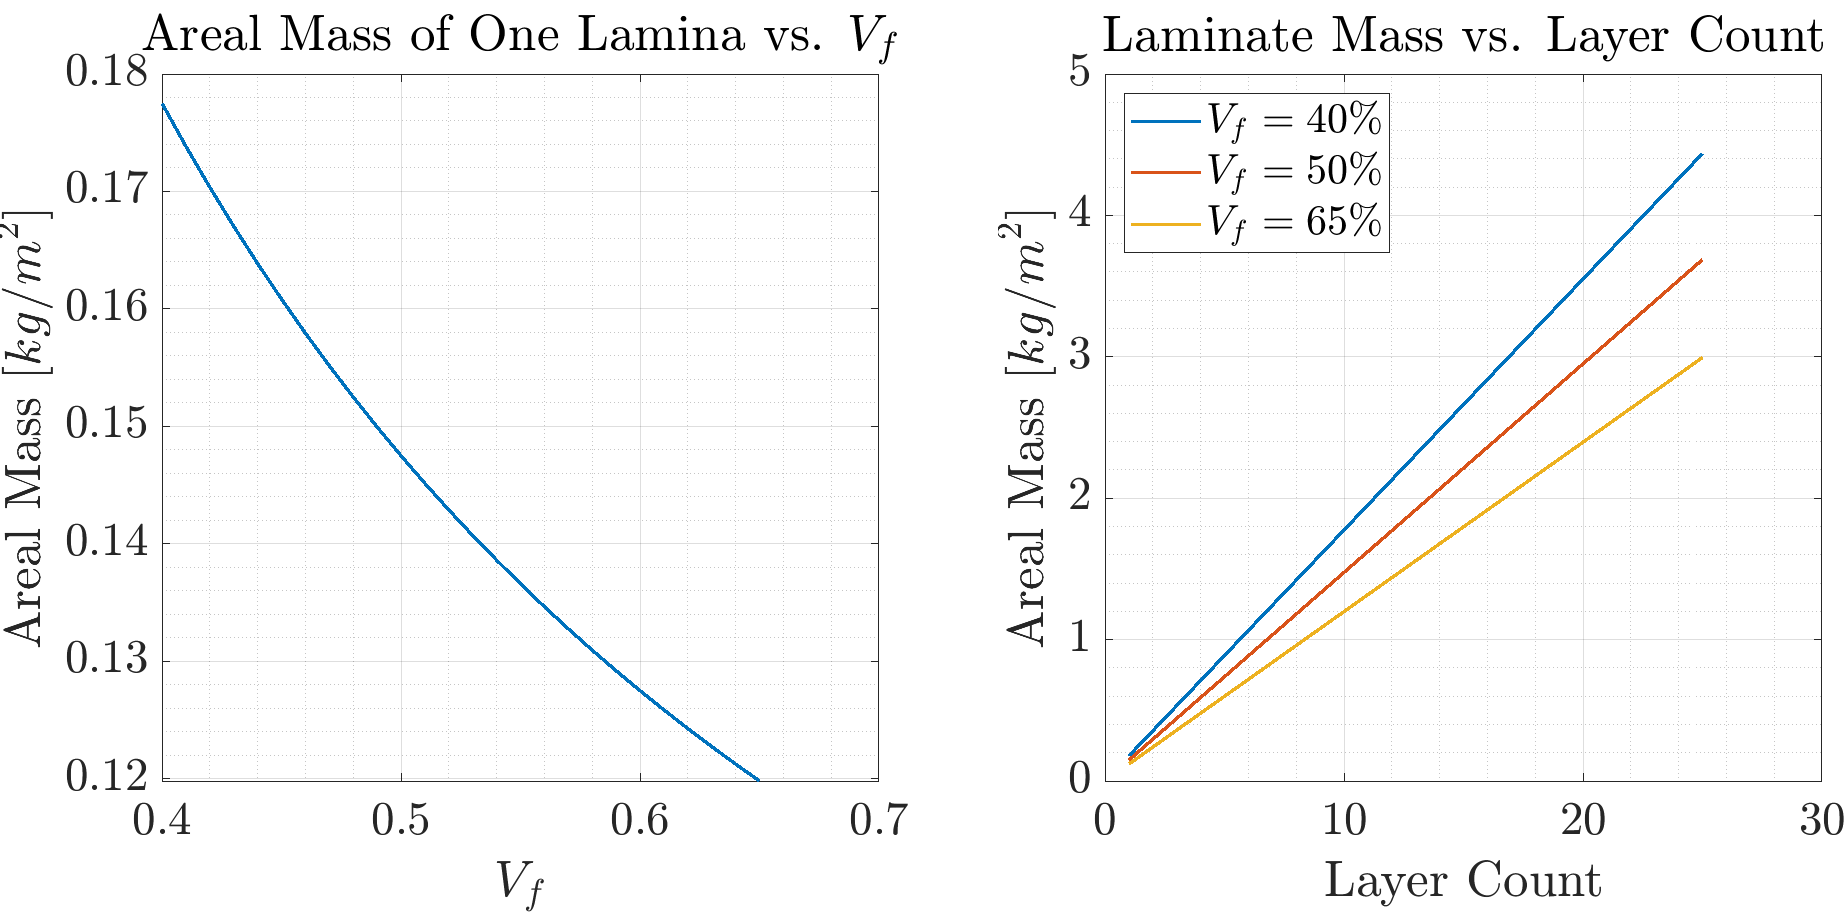
\includegraphics[width=0.99\linewidth]{massChange.png}
    \caption{Laminate mass depends more on laminate count than $V_f$}
    \label{fig:massChange}
\end{figure}



\section{Designing for Stiffness}

The criteria provided for the stiffness based design are as follows:

\begin{equation}
  \begin{aligned}
    A_{xx} &\geq 100,000 \text{ N/mm} & A_{\overline{xx}} &\geq 30,000 \text{ N/mm} \\ %\text{ N/mm, in the main x-y reference frame} \\
     % \\ % \text{ N/mm, all rotations of the main reference frame into a different reference frame.} \\
    D_{xx} &\geq 25,000 \text{ N/mm} & D_{yy} &\geq 15,000 \text{ N/mm}
    \label{eq:stiffness}
  \end{aligned}
\end{equation}


We built a function that took an ABD matrix as the input and output a boolean pass or fail for each of the above criteria. This allowed us to quickly build laminates, create the ABD, and test them. Only laminates that passed all 4 criteria are considered.

In order to find the most optimal laminate, we created a program that used a vector of possible lamina directions, in most cases this was $-75^\circ$ to $90^\circ$ in increments of $15^\circ$. The laminas were then arranged into the following structure:

\begin{equation*}
    [\theta _1 / \theta_2/\theta_3/ .../\theta_3/\theta_2/\theta_1]
\end{equation*}

All of these laminates were assumed to be symmetric, both to avoid coupling and to ease computational requirements, and MATLAB \mcode{parfor} was used to speed up computation as none of the calculations depend on each other. 

We began by building 16-ply quasi-isotropic laminates that satisfied the requirements. This provided an idea of where we should start. The simplest way to minimize the weight is to reduce the number of layers. So we went down to 10, generating all possible laminates using our layup and angles defined earlier. These were tested at volume fractions of $40 \%$ and $65 \%$. None passed, so we moved up to 11 ply, then 12. Finally, at 13 we began returning successful laminates. 

All of these successful laminates included 0's at the edges and the center along with 90 degree laminas just inside of the outer edge. Using this information we went back to the 12 laminate case, setting values for the center and the edges as follows:

\begin{equation*}
    [0/90/\theta _1 / \theta_2/\theta_3/ 0/\theta_3/\theta_2/\theta_1/90/0]
\end{equation*}

The test resolution was then increased to $5^\circ$ and then to $1^\circ$ to see if we could once again reduce the plies and find a working laminate. After testing over 10 million different configurations across a variety of angles and volume fractions and returning no results, we have resigned ourselves to saying the lightest laminate we can find with this technique will be 13 plies thick.

These laminates only work at $40\%$ volume fraction (even increasing to $41\%$ causes them to fail), this is because a lower $V_f$ makes the laminate overall slightly thicker, increasing the values in the $D$ matrix where distance from the neutral axis is cubed. 

At this point, when we have set that we are using 13 plies at $40\%$ volume fraction, the exact configuration we choose from our list does not matter. They all weigh the same and are all part of that list because they have satisfied the four requirements, so we select the following for its simplicity:

\begin{equation*}
    [0   / 90   /  0  /  75  /   0  /   0   /  0  /   0  /   0  /  75  /   0 /   90  /   0]
\end{equation*}

Finally, we calculate the weight of this laminate. Because it is not the $50 \%$ volume fraction specified for $0.1\;mm$ lamina thickness, we must first calculate the corresponding thickness for a $40 \% $ volume fraction. This is done using the following equation:

\begin{equation}
    \text{Lamina Thickness }t =  \frac{\text{Fiber Thickness}}{V_f}
    \label{eq:tv}
\end{equation}

Using the example case, the fiber thickness is calculated to be $0.05\;mm$. We can then proceed to find that that the lamina thickness at $40 \%$ volume fraction is $0.125\;mm$. 

The Rule of Mixtures is used to calculate the effective density of the whole composite:

\begin{equation*}
    \rho = V_f \rho _f + (1-V_f) \rho_m
\end{equation*}

\begin{framed}
Now with our effective density ($1420 \; kg/m^3$), lamina heights ($0.125\;mm$), and lamina count (13), we can calculate that the lightest laminate we designed to satisfy all four stiffness requirements weighs $2.31\;kg/m^2$.
    
\end{framed}

\section{Designing for Strength}
\label{sec:strength}

\subsection{Lamina Failure Criteria}

To determine the failure criteria for each lamina, we calculated the failure strengths in the 1 and 2 directions for tension ($F_{1t}$, $F_{2t}$) and compression ($F_{1c}$, $F_{2c}$), along with shear failure strength ($F_6$). Using the equations below (Daniel and Ishai, Chapter 5), we were able to find failure strengths based on the failure parameters provided for the individual material components, with $V_f$ as the only parameter subject to change.

\begin{multicols}{2}
\begin{align}
    F_{1t} &= \varepsilon_{f}^{u}E_{1f}\left(V_f+(1-V_f)\frac{E_m}{E_{1f}}\right)\\
    F_{2t} &= F_{mt} \frac{1-\left( \frac{E_m}{E_{2f}}\sqrt{\frac{4V_f}{\pi}} \right)}{1-V_f\left(1-\frac{E_m}{E_{2f}}\right)}\\
    F_{1c} &= 2V_f\sqrt{\frac{E_mE_{1f}V_f}{3(1-V_f)}}
\end{align}
\begin{align}
    F_{2c} &= F_{mc} \frac{1-\left( \frac{E_m}{E_{2f}}\sqrt{\frac{4V_f}{\pi}} \right)}{1-V_f\left(1-\frac{E_m}{E_{2f}}\right)}\\ 
    F_6 &= F_{ms} \frac{1-\left( \frac{G_m}{G_{12f}}\sqrt{\frac{4V_f}{\pi}} \right)}{1-V_f\left(1-\frac{G_m}{G_{12f}}\right)}
\end{align}
\end{multicols}

\subsection{Determining viable layups through direct computation}

In much the same way as when designing for stiffness, we selected a layup design to meet the strength criteria (shown below) by simply iterating through possible combinations of lamina count and lamina fiber angle, checking each against the strength criteria, until we found several possible designs.

% \begin{multicols*}{3}
%     \begin{equation*}
%         N_{xx} = 600 N/mm
%     \end{equation*}
%     \begin{equation*}
%         N_{\theta \theta}= 200 N/mm
%     \end{equation*}
%     \begin{equation}
%         M_{xx} = \pm 100 N
%         \label{eq:strength}
%     \end{equation}
% \end{multicols*}

\begin{equation}
  \begin{aligned}
    N_{xx} = 600 N/mm &   \;\; N_{\theta \theta} = 200 N/mm & M_{xx} = \pm 100 N
    \label{eq:strength}
  \end{aligned}
\end{equation}

We began our search using relatively low lamina counts, iterating through choices using nested \mcode{for} loops. This method was sufficient to rule out laminates with as many as 10 or so lamina, at which point the additional compute time to check $n+1$ laminas became prohibitively long.

In pursuit of the ability to brute-force check all possible angle combinations for laminates with higher lamina counts, several improvements were made to increase the computational efficiency of the code. The first step was to turn a deep nested \mcode{for} loop into something that could be run in parallel; just as in the stiffness case the calculations for each layup do not depend on each other and so can be run in parallel. This is achieved by using the Parallel Computing Toolbox from MATLAB. Listing \ref{lst:broadcast} shows an example of what this looks like. This technique is faster than a normal \mcode{for} loop but has serious draw backs. The way it is set up, the \mcode{theta} variable is a "broadcast" variable, meaning it doesn't change with each loop and gets sent to all of the parallel workers. This slows down the operation a decent amount.

% \begin{framed}
%     \label{frame:broadcast}
%     \centerline{\textbf{\mcode{parfor} loop with broadcast $\theta$ variable}}
%     \skipline
\begin{lstlisting}[label=lst:broadcast,caption=\mcode{parfor} loop with a broadcast variable]
dt = 15
theta = (-90 + dt):dt:90; 
parfor a = 1:leng
    for b = 1:leng
        ...
            for g = 1:leng
                layup = deg2rad([thetas(a), thetas(b),thetas(c),thetas(d), thetas(e) 0, 0, 0, thetas(e), thetas(d), thetas(c), thetas(b), thetas(a)]);
                
                pass = strengthCheck(layup);

            end
        ...          
    end
end
\end{lstlisting}
% \end{framed}

We can avoid using broadcast variables by pre-computing all possible combinations of $\theta$ values (this happens in the \mcode{build_angle_combos.m} function in the project repository), and then running the strength check in a single \mcode{parfor} loop, as shown in Listing \ref{lst:oneloop}. Also worth noting in this code block is the use of \mcode{n_fill}, which determines the number of middle layers that should be left un-calculated. We found that generally speaking leaving the middle 3 or 4 layers as $0^\circ$ lamina for the stiffness case and $90^\circ$ lamina for the strength case greatly decreased the number of variations we needed to check without missing too many of the viable options. By fixing more laminas, we decrease the number of combinations that need to be checked. The number of combinations, $N$, depends on the number of $\theta$ values to be searched, $k$, and the number of lamina being varied, $n$: $N = k^n$. $N$ goes up  with increases to both $k$ and $n$, so keeping both low is desirable, even though doing so limits the variability of designs being checked, decreasing our chances of finding a best case design.


\begin{lstlisting}[label=lst:oneloop,caption=\mcode{parfor} loop with precomputed angle combinations]
    [angle_combinations, num_combinations] = build_angle_combos(thetas, n, n_fill);
    count = 0;
    winners = [];
    parfor i = 1:num_combinations
        layup_angles = angle_combinations(i, :);
    
        % Construct the layup with varying and fixed angles
        layup = deg2rad([layup_angles, mid_layers, layup_angles(end:-1:1)]);
    
        [Pass] = strengthCheck(layup, V_f);

        if Pass
            count = count + 1;
            winners = [winners;rad2deg(layup)];
        end
    end
\end{lstlisting}

The above method was sufficient for direct computing every layer of 10-15 lamina thick layup designs, but yielded no designs that passed the strength requirements. In order to speed up computation even more, the above method was compiled into \texttt{C} code functions callable from in MATLAB (These are the \mcode{.mex} files in the project repository). Simply compiling to \texttt{C} and running the checks that way sped up the process enough to check every layer of a 16-lamina layup at angular step sizes of $\Delta \theta = 30^\circ$. Smaller steps sizes could run within human time frames, but fail in a new way: integer size limits. Array sizes in \texttt{C} are limited (at least for computer science novices) by the maximum integer value of 2,147,483,647. Some how, for $N = 12^8 = 429,981,696$, an array in the \texttt{C} code breaches this size limit, and the code errors. This is possibly because for each lamina, the strength check requires rotating the laminate through $\theta = 0^\circ\rightarrow90^\circ$, meaning there are around $3.87\times10^{10}$ calculations, which is much more than the $2.15\times10^9$ limit. An increment of $\Delta \theta = 20^\circ$ requires $3.9\times10^9$ calculations, An increment of $\Delta \theta = 25^\circ$ requires only $5.2\times 10^8$ calculations, but yields no new results; in fact, using a step size of $\Delta \theta = 45^\circ$ yields identical results; decreasing step size past that doesn't improve things for us.

\subsection{The lightest solution}

The code discussed above yields three 16 ply laminate designs that pass the strength criteria, they are shown in Equation \ref{eq:16ply}. The variations here are small, with just one zero/ninety combination hopping around on the inner layers. All of the outer layers are zero plys, which is a big difference from the lightest designs for the stiffness criteria, which benefited from having zero plys in the middle and angle plys on the outside to help with the $D_{yy}$ stiffness value.

\begin{equation}
    \begin{aligned}
        [0/0/0/0/0/0/90/90]_s \\
        [0/0/0/0/0/90/0/90]_s \\
        [0/0/0/0/0/90/90/0]_s
        \label{eq:16ply} 
    \end{aligned}
\end{equation}

These three lamina all work at $V_f = 65\%$, which is ideal for minimizing the mass of the laminate. The first option worked at the lowest volume fraction of the three, $V_{f,min} = 49\%$. As an example of how we worked through our options, we can compare the first solution and the third solution on how they do with the Tsai-Wu failure criteria. Figure \ref{fig:op3} shows the third solution simulated with a low volume fraction; it just barely fails the Tsai-Wu Criteria in the eleventh ply. Figure \ref{fig:strong} shows the first option at the same volume fraction; it passes nicely. 

In all cases with the strength checks, the criteria skew higher towards the top of the lamina. This is because we are only simulating a positive bending moment, and so the higher number lamina are experiencing the highest tension stresses. The laminates are all symmetric, and so also pass the criteria for a negative bending moment.

\begin{figure}[H]
    \centering
    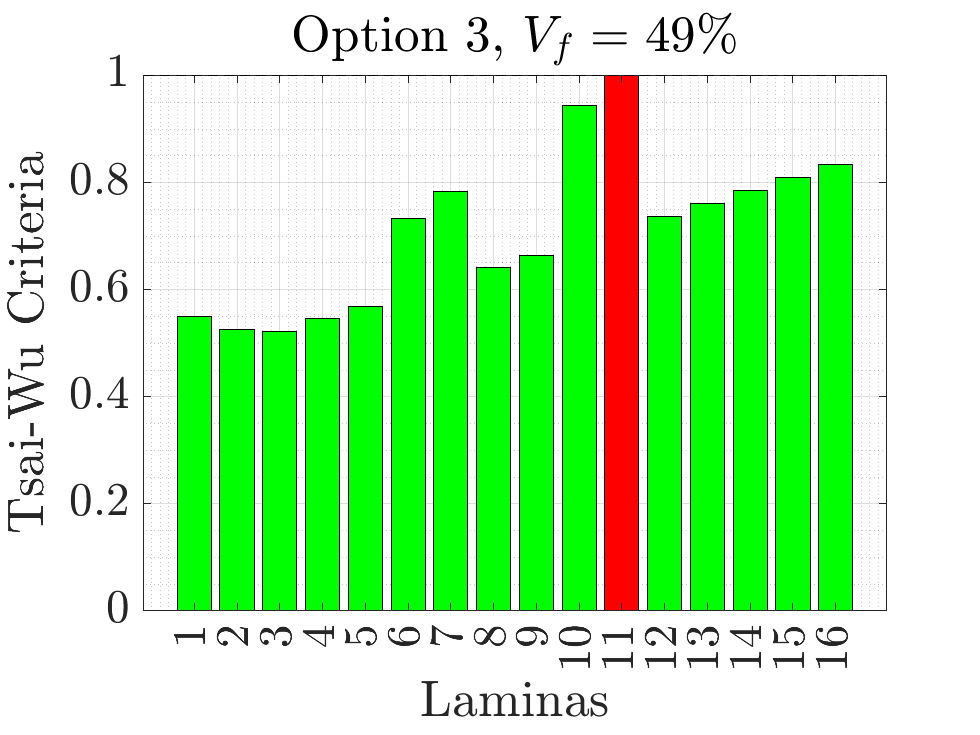
\includegraphics[width=0.75\linewidth]{op3fails.png}
    \caption{The laminate with $0^\circ$ inner plys fails the criteria with $V_f = 49\%$, but only on one ply.}
    \label{fig:op3}
\end{figure}

\begin{figure}[H]
    \centering
    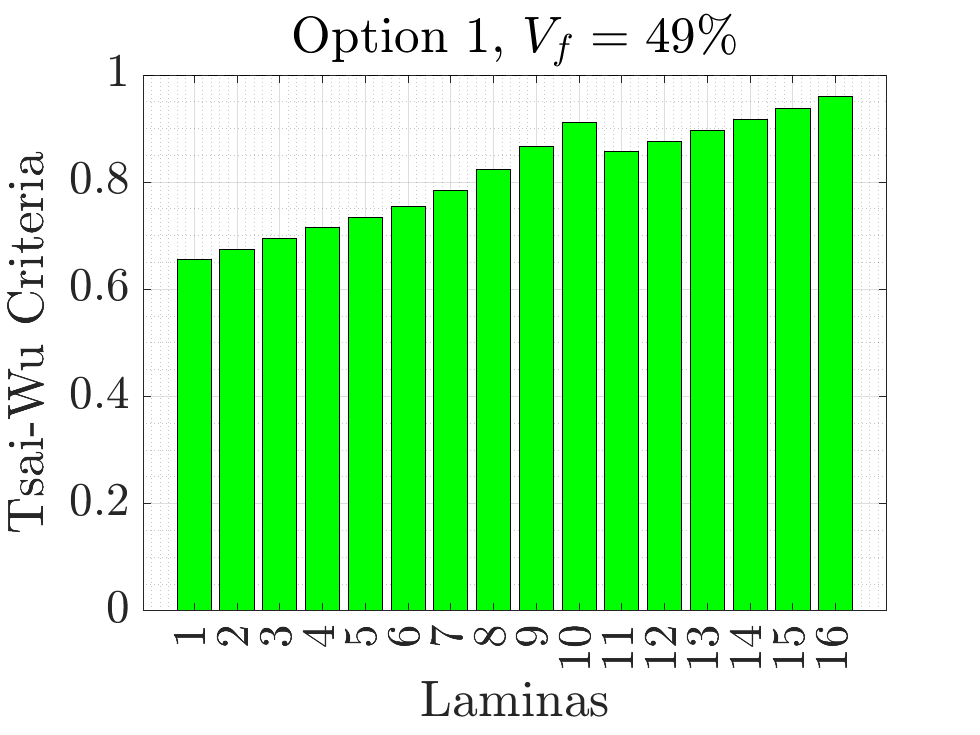
\includegraphics[width=0.75\linewidth]{stronglaminate.png}
    \caption{The laminate with $90^\circ$ inner plys passes with $V_f = 49\%$}
    \label{fig:strong}
\end{figure}


Because lower volume fractions can help with satisfying the stiffness criteria, we like this laminate the most due to it's relative flexibility in terms of viable volume fractions. 



\begin{framed}
The lightest overall laminate that satisfies the strength criteria is a 16-ply laminate with $V_f = 0.65$ with any of the layup schedules listed in Equation \ref{eq:16ply}. These laminates, aided by their higher volume fractions, weigh only 1.92 $kg/m^2$
\end{framed}

% \begin{multicols}{2}
    
%     \begin{framed}
%         test 2
%     \end{framed}
% \end{multicols}

\section{¿Por que no los dos? Design for Stiffness \& Strength}

Our last objective was to find the lightest laminate that could simultaneously satisfy both the Stiffness (Equation \ref{eq:stiffness}) and the Strength (Equation \ref{eq:strength}) criteria. We started with our 16-ply laminate from Section \ref{sec:strength} at the lower $49 \%$ volume fraction. While this obviously passed the Strength criteria, it failed in Stiffness. We then expanded our search to $1\%$ steps of volume fraction on the same laminate, which failed in all cases.

Next, we included all 3 of the laminates found to satisfy the Strength requirements, and allowed volume fraction to vary from $40\%$ to $65\%$. Many of these options got close: satisfying all stiffness but not strength or satisfying strength and 3 of the 4 stiffness requirements. None of them were successful across all the criteria.

We now once again open up our design space to all 16-ply composites. Lamina rotations are changed as before at a step size of $15 ^\circ$ and volume fractions are incremented by $1 ^\circ$ from $40\%$ to $65\%$. No working laminates are found at 16, 17, or 18 plies.

Exceeding 18 plies slowed even our most efficient code to a halt. At this point, we applied what we had learned in the previous two sections to build our own layups by hand. We know that the $A_{xx}$ criteria just requires at least eight $0 ^\circ$ plies to exist in the laminate. $A_{\overline{xx}} $ then requires some amount of positive and negative angled ply or $90 ^\circ$ lamina. $D_{xx}$ increases as $0 ^\circ$ plies are moved towards the outer edges of the laminate, with the same happening to $D_{yy}$ and $90 ^\circ$. While the $N_{xx}$ and $N_{\theta \theta}$ restrictions proved simple to meet, the difficulty lay in $M_{xx}$. As total laminate thickness increases, the strain experienced increases by a power of 3 to the distance from the center of the laminate. This causes the lamina on the outside of the laminate to fail in most bending scenarios. Most of the criteria favored a lower volume fraction ($40 \%$).

Using these lessons and our Strength optimized laminate as our starting point, we finally settled on the following 21-ply laminate to satisfy both the Stiffness and Strength requirements:

\begin{gather*}
        [90/ 0 /0 /0/ 0/ 0/ 0/ 0/ 0/ 90/ 90/ 90/ 0/ 0/ 0/ 0/ 0/ 0/ 0/ 0/ 90] \\
        \text{or} \\
        [90/ 0 /0 /0/ 0/ 0/ 0/ 0/ 0/ 90/ \overline{90}]_s
        \label{eq:21ply} 
\end{gather*}

\begin{framed}

Composed of 21 laminas at a volume fraction of $40 \%$, this composite is $3.73 \; kg/m^2$, the lightest that we found that satisfies both the stiffness and strength criteria.

\end{framed}

\section{Future Work and Conclusion}




In order to validate that all of these choices truly are the lightest possible composites that satisfy the given requirements, a more robust numerical approach is needed. What began as a brute force method in MATLAB evolved into a more efficient process in compiled \texttt{C} code. However, a better choice from the start would have been a multi-dimensional gradient descent model or the use of a minimizer like MATLAB's \mcode{fmincon}. In both of these cases, a provided starting guess is improved on by altering inputs in a way that shift the solution to a more successful location. This would have prevented a lot of wasted time testing laminates that satisfied none of the requirements or laminates that were very similar to each other.

Given more time on this project, we would choose to use one of the two options listed above to test lighter options with more resolution. Step sizes of $30 ^\circ$ were too coarse to confidently say that there were zero laminates at lower lamina counts that satisfied the requirements. 

Finally, it is worth noting that our primary method of minimizing mass was reducing $n$. Given the relationship between $n$, $V_f$, and mass, it is possible that there is a solution with more layers that allows for a significant enough adjustment to $V_f$ to produce a lower areal mass. Considering our less efficient methods discussed above, these increases were often impractical and those options were not tested. Had we arrived at a more clever method for searching solution spaces, we would have liked to explore this idea in greater depth.

Table \ref{tab:results} is a summary of our chosen designs for each section of the project. For detail on all of the code written for this project, please visit the project \href{https://github.com/brycepfuetze/ASEN-5212-Composites-Project.git}{GitHub repository} to view the \mcode{README.md} or read through individual functions and scripts.

\begin{table}[H]
    \centering
    \begin{tabular}{|c|c|c|c|c|}
        \hline
        \textbf{Case} & \textbf{Laminate} & $\boldsymbol{V_f}$ & \textbf{Areal mass} $\boldsymbol{[\frac{kg}{m^2}]}$ & \textbf{Ply Count} \\
        \hline
        Stiffness & $[0/90/0/75/0/0/\bar{0}]_s$ & 0.4 & 2.3075 & 13 \\
        \hline
         & $[0/0/0/0/0/0/90/90]_s$ &  & &\\
        Strength & $[0/0/0/0/0/90/0/90]_s$ & 0.65 & 1.92 & 16\\
         & $[0/0/0/0/0/90/90/0]_s$ &  & &\\
        \hline
        Both & $[90/0/0/0/0/0/0/0/0/90/\bar{90}]_s$ & 0.4 & 3.7275 & 21\\
        \hline
    \end{tabular}
    \caption{Chosen laminates for each case}
    \label{tab:results}
\end{table}

\end{document}
